\section{成员选择与集成简化}
\label{sec:ensemble-selection-compression}

Bagging、Boosting和Stacking先回答怎样形成组合。部署时，多成员推理可能超出内存或延迟预算，一些成员也可能只在局部输入上有用。简化集成有三种不同目标：为所有输入固定一个较小成员子集，针对当前输入临时选择成员，或训练一个新的紧凑模型替代原集成。前两种方法保留部分原成员，第三种方法改变了部署模型。

图\ref{fig:ensemble-selection-compression}沿部署对象区分这三种目标。静态选择把成员池缩成一个固定子集，动态选择保留成员池并让路由依赖当前输入，紧凑化则把完整集成的行为转移到新模型。资源评价据此包括被部署模型以及选择或路由计算。

\begin{figure*}[htbp]
  \centering
  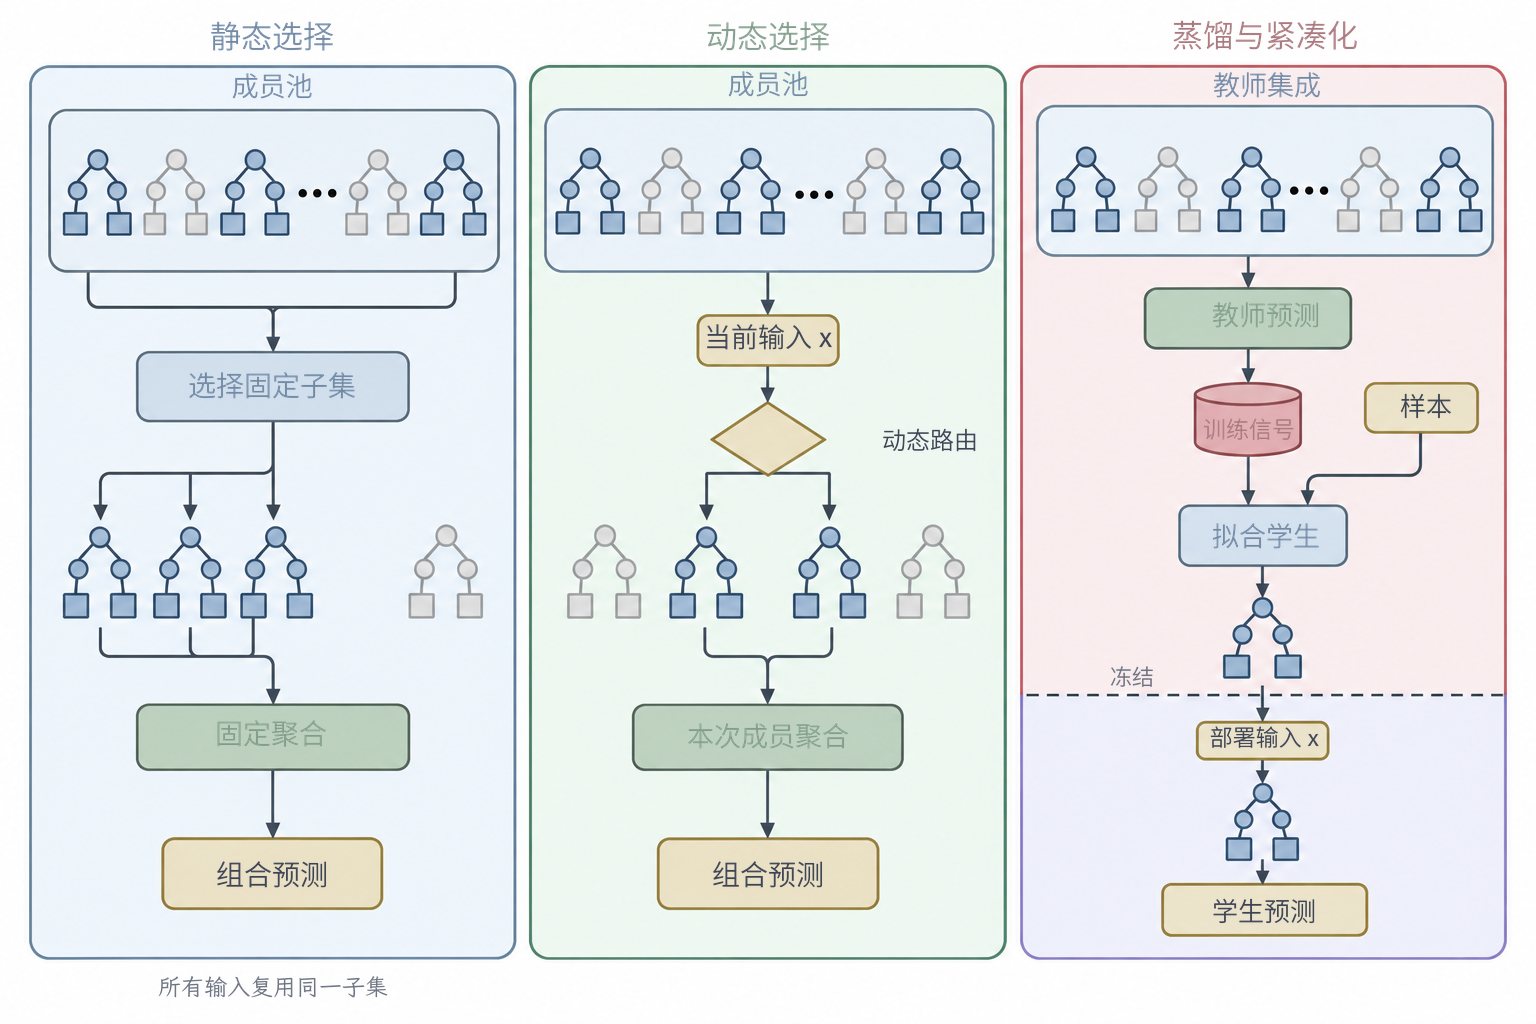
\includegraphics[width=130.048mm]{figures/04-classic-models/00-shared/generated/ensemble-selection-compression/figure.png}
  \caption{静态成员选择、动态成员选择与紧凑化改变的部署对象。静态选择为所有输入保留同一成员子集；动态选择根据输入改变运行成员或组合权重；紧凑化训练并部署新的学生模型。三种路径改变的计算对象不同，成本需沿各自完整路径测量。}
  \label{fig:ensemble-selection-compression}
\end{figure*}

\subsection{静态成员选择}
\label{sec:ensemble-static-selection}

\subsubsection{模型结构}

部署时若只能保留部分成员，我们需要选择在预算内预测效果合适的组合。单模型评分还不足以作出选择：几份预测近乎相同的强成员可能互相重复，加入一个单独误差稍大、但能纠正它们共同错误的成员，反而可能得到更好的组合。\term{静态成员选择}（static ensemble selection）从已经训练好的候选池$\{h_1,\ldots,h_M\}$中，选择一个对所有未来输入都相同的非空子集$S\subseteq\{1,\ldots,M\}$，评价对象是整个子集的组合预测。

\subsubsection{参数学习}

若$\mathcal{L}_{\mathrm{val}}(S)$表示该组合的平均验证损失，可以用损失与部署成本共同选择子集：
\begin{equation}
  \widehat{S}
  \in
  \argmin_{\varnothing\neq S\subseteq\{1,\ldots,M\}}
  \mathcal{L}_{\mathrm{val}}(S)
  +\lambda_1|S|
  +\lambda_2 C(S),
  \label{eq:ensemble-static-selection}
\end{equation}
其中$\lambda_1,\lambda_2\geq0$，$|S|$控制成员数，$C(S)$可以表示存储、单样本延迟或其他部署成本。成员池包含指数多个子集，实际可用排序、逐个加入或删除等方法近似搜索，并记录所得子集的验证损失与资源成本。

单成员排序忽略预测的重叠，可能同时保留许多相似模型。前向选择则评价候选加入当前组合后的损失变化，使选择依赖已有成员。允许重复选择某个成员时，重复次数还形成离散权重。基于模型库的贪心集成选择就是这种做法的代表：从一个初始组合出发，每轮加入使验证指标改善最大的候选，必要时使用多起点或装袋法减少搜索的不稳定性\scite{caruana2004ensemble}。

式\eqref{eq:ensemble-static-selection}的搜索对象为固定池中的成员子集，成员预测已经形成。若同时改变基学习算法、特征处理和超参数，搜索范围已经扩展为完整模型开发流程。候选池越大，验证集上偶然出现有利组合的机会也越多；最终测试需在该子集及其组合规则固定后进行。

\subsection{动态成员选择}
\label{sec:ensemble-dynamic-selection}

\subsubsection{模型结构}

静态方案让所有输入使用相同子集，却可能遗漏成员能力随输入改变的情况。假设一个文本分类器在体育报道附近的预测可靠，另一个在科技报道附近更可靠，用全体文档上的平均正确率排序，就可能忽略这种局部差别。我们可以在独立数据中寻找与当前输入邻近的记录，比较成员在这些记录上的表现，再决定调用谁。\term{动态分类器选择}（dynamic classifier selection, DCS）为每个输入选择一个成员；\term{动态集成选择}（dynamic ensemble selection, DES）选择一个成员子集或给出输入相关权重。

\subsubsection{参数学习}

一种基本构造是准备独立的能力估计数据。对查询输入$\bm{x}$，在该数据中寻找非空邻域$\mathcal{N}(\bm{x})$，再以成员$m$在邻域内的正确率估计
\begin{equation}
  \widehat{c}_m(\bm{x})
  =
  \frac{1}{|\mathcal{N}(\bm{x})|}
  \sum_{i\in\mathcal{N}(\bm{x})}
  \mathbb{I}\!\left\{h_m(\bm{x}_i)=y_i\right\}.
  \label{eq:ensemble-local-competence}
\end{equation}
DCS可以选择$\widehat{c}_m(\bm{x})$最大的成员，DES则保留超过阈值的成员或按能力加权。局部正确率只是能力估计的一种方式，还可以使用输出轮廓、分类间隔或由元模型学习的能力特征\scite{woods1997localaccuracy}。

局部选择依赖邻域和能力估计两部分。邻域依赖输入表示与距离，高维或分布稀疏时，附近样本未必提供稳定的局部证据；能力估计器也可能在有限数据上过拟合。成员训练数据、能力估计数据与最终测试数据需要分开，所有标准化和邻域参数都在相应开发流程内确定。

动态选择的延迟由路由和实际运行成员共同决定。若系统必须先运行全部成员才能构造输出轮廓，再选择其中几个聚合，选择之前已经支付全部成员计算；基于输入邻域的方法还增加了检索成本。在昂贵成员运行前完成路由，才可能直接省去被跳过成员的计算；局部检索、路由和输出质量需要一并测量。

\subsection{从集成模型到紧凑模型}
\label{sec:ensemble-compression}

\subsubsection{模型结构}

若原成员的最小可用子集仍超预算，可以另外训练一个新的\term{紧凑模型}（compact model），使其逼近完整集成的输入输出映射。早期模型压缩工作已经用大型集成的输出训练较小模型；知识蒸馏随后把这种教师到学生的传递扩展为常用训练形式\scite{bucilua2006compression,hinton2015distilling}。

\subsubsection{参数学习}

设完整集成为教师$H$，紧凑模型为学生$s_{\bm{\theta}}$。对回归，可以组合真实响应损失与教师拟合损失：
\begin{equation}
  \min_{\bm{\theta}}
  \sum_{i=1}^{n}
  \left[
    \alpha\ell\!\left(y_i,s_{\bm{\theta}}(\bm{x}_i)\right)
    +(1-\alpha)
    \ell\!\left(H(\bm{x}_i),s_{\bm{\theta}}(\bm{x}_i)\right)
  \right],
  \label{eq:ensemble-compression-objective}
\end{equation}
其中$\alpha\in[0,1]$控制真实标签与教师输出的作用。分类时可以拟合教师的完整类别分布；温度缩放会使非最大类别之间的相对关系更容易进入训练信号，但温度、损失权重与部署概率仍须分别选择和校准。

学生训练输入可以来自原训练集、额外未标注样本或经过说明的合成样本。教师在所选输入上提供训练目标；覆盖不足的区域缺少这种监督，学生在这些区域仍可能偏离教师。学生容量过小会产生逼近误差，容量很大则可能无法达到预期资源节省。
